% Graphic for TeX using PGF
% Title: /home/jnicolaschc/GitHub/Teoría de Telecominicaciones I /ttl1_trabajo3/Documentos/desarrollo/codigofuente/pgf/trapezoide.dia
% Creator: Dia v0.97+git
% CreationDate: Sat Aug 21 00:36:32 2021
% For: jnicolaschc
% \usepackage{tikz}
% The following commands are not supported in PSTricks at present
% We define them conditionally, so when they are implemented,
% this pgf file will use them.
\begin{figure}[H]
	\centering
	\ifx\du\undefined
		\newlength{\du}
	\fi
	\setlength{\du}{15\unitlength}
	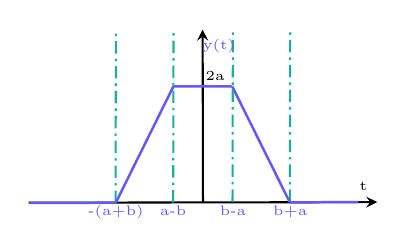
\begin{tikzpicture}[scale = 0.7]
		\pgftransformxscale{1.000000}
		\pgftransformyscale{-1.000000}
		\definecolor{dialinecolor}{rgb}{0.000000, 0.000000, 0.000000}
		\pgfsetstrokecolor{dialinecolor}
		\pgfsetstrokeopacity{1.000000}
		\definecolor{diafillcolor}{rgb}{1.000000, 1.000000, 1.000000}
		\pgfsetfillcolor{diafillcolor}
		\pgfsetfillopacity{1.000000}
		\pgfsetlinewidth{0.050000\du}
		\pgfsetdash{}{0pt}
		\pgfsetbuttcap
		{
			\definecolor{diafillcolor}{rgb}{0.000000, 0.000000, 0.000000}
			\pgfsetfillcolor{diafillcolor}
			\pgfsetfillopacity{1.000000}
			% was here!!!
			\pgfsetarrowsend{stealth}
			\definecolor{dialinecolor}{rgb}{0.000000, 0.000000, 0.000000}
			\pgfsetstrokecolor{dialinecolor}
			\pgfsetstrokeopacity{1.000000}
			\draw (44.008667\du,15.010903\du)--(56.001842\du,14.989880\du);
		}
		\pgfsetlinewidth{0.050000\du}
		\pgfsetdash{}{0pt}
		\pgfsetbuttcap
		{
			\definecolor{diafillcolor}{rgb}{0.000000, 0.000000, 0.000000}
			\pgfsetfillcolor{diafillcolor}
			\pgfsetfillopacity{1.000000}
			% was here!!!
			\pgfsetarrowsend{stealth}
			\definecolor{dialinecolor}{rgb}{0.000000, 0.000000, 0.000000}
			\pgfsetstrokecolor{dialinecolor}
			\pgfsetstrokeopacity{1.000000}
			\draw (50.005254\du,15.000392\du)--(49.993900\du,9.052460\du);
		}
		\pgfsetlinewidth{0.050000\du}
		\pgfsetdash{{0.300000\du}{0.120000\du}{0.060000\du}{0.120000\du}}{0cm}
		\pgfsetbuttcap
		{
			\definecolor{diafillcolor}{rgb}{0.101961, 0.682353, 0.623529}
			\pgfsetfillcolor{diafillcolor}
			\pgfsetfillopacity{1.000000}
			% was here!!!
			\definecolor{dialinecolor}{rgb}{0.101961, 0.682353, 0.623529}
			\pgfsetstrokecolor{dialinecolor}
			\pgfsetstrokeopacity{1.000000}
			\draw (46.996400\du,15.021100\du)--(47.008100\du,9.063880\du);
		}
		\pgfsetlinewidth{0.050000\du}
		\pgfsetdash{{0.300000\du}{0.120000\du}{0.060000\du}{0.120000\du}}{0cm}
		\pgfsetbuttcap
		{
			\definecolor{diafillcolor}{rgb}{0.101961, 0.682353, 0.623529}
			\pgfsetfillcolor{diafillcolor}
			\pgfsetfillopacity{1.000000}
			% was here!!!
			\definecolor{dialinecolor}{rgb}{0.101961, 0.682353, 0.623529}
			\pgfsetstrokecolor{dialinecolor}
			\pgfsetstrokeopacity{1.000000}
			\draw (48.980200\du,15.007400\du)--(48.992000\du,9.050250\du);
		}
		\pgfsetlinewidth{0.050000\du}
		\pgfsetdash{{0.300000\du}{0.120000\du}{0.060000\du}{0.120000\du}}{0cm}
		\pgfsetbuttcap
		{
			\definecolor{diafillcolor}{rgb}{0.101961, 0.682353, 0.623529}
			\pgfsetfillcolor{diafillcolor}
			\pgfsetfillopacity{1.000000}
			% was here!!!
			\definecolor{dialinecolor}{rgb}{0.101961, 0.682353, 0.623529}
			\pgfsetstrokecolor{dialinecolor}
			\pgfsetstrokeopacity{1.000000}
			\draw (51.022200\du,14.980200\du)--(51.033900\du,9.022980\du);
		}
		\pgfsetlinewidth{0.050000\du}
		\pgfsetdash{{0.300000\du}{0.120000\du}{0.060000\du}{0.120000\du}}{0cm}
		\pgfsetbuttcap
		{
			\definecolor{diafillcolor}{rgb}{0.101961, 0.682353, 0.623529}
			\pgfsetfillcolor{diafillcolor}
			\pgfsetfillopacity{1.000000}
			% was here!!!
			\definecolor{dialinecolor}{rgb}{0.101961, 0.682353, 0.623529}
			\pgfsetstrokecolor{dialinecolor}
			\pgfsetstrokeopacity{1.000000}
			\draw (52.996000\du,14.980200\du)--(53.007700\du,9.022980\du);
		}
		\pgfsetlinewidth{0.060000\du}
		\pgfsetdash{}{0pt}
		\pgfsetbuttcap
		{
			\definecolor{diafillcolor}{rgb}{0.396078, 0.345098, 0.960784}
			\pgfsetfillcolor{diafillcolor}
			\pgfsetfillopacity{1.000000}
			% was here!!!
			\definecolor{dialinecolor}{rgb}{0.396078, 0.345098, 0.960784}
			\pgfsetstrokecolor{dialinecolor}
			\pgfsetstrokeopacity{1.000000}
			\draw (44.028502\du,15.015292\du)--(46.988200\du,15.011200\du);
		}
		\pgfsetlinewidth{0.060000\du}
		\pgfsetdash{}{0pt}
		\pgfsetbuttcap
		{
			\definecolor{diafillcolor}{rgb}{0.396078, 0.345098, 0.960784}
			\pgfsetfillcolor{diafillcolor}
			\pgfsetfillopacity{1.000000}
			% was here!!!
			\definecolor{dialinecolor}{rgb}{0.396078, 0.345098, 0.960784}
			\pgfsetstrokecolor{dialinecolor}
			\pgfsetstrokeopacity{1.000000}
			\draw (47.011200\du,14.999700\du)--(48.992089\du,10.999108\du);
		}
		% setfont left to latex
		\definecolor{dialinecolor}{rgb}{0.396078, 0.345098, 0.960784}
		\pgfsetstrokecolor{dialinecolor}
		\pgfsetstrokeopacity{1.000000}
		\definecolor{diafillcolor}{rgb}{0.396078, 0.345098, 0.960784}
		\pgfsetfillcolor{diafillcolor}
		\pgfsetfillopacity{1.000000}
		\node[anchor=base,inner sep=0pt, outer sep=0pt,color=dialinecolor] at (47.009500\du,15.451675\du){\tiny -(a+b)};
		% setfont left to latex
		\definecolor{dialinecolor}{rgb}{0.396078, 0.345098, 0.960784}
		\pgfsetstrokecolor{dialinecolor}
		\pgfsetstrokeopacity{1.000000}
		\definecolor{diafillcolor}{rgb}{0.396078, 0.345098, 0.960784}
		\pgfsetfillcolor{diafillcolor}
		\pgfsetfillopacity{1.000000}
		\node[anchor=base,inner sep=0pt, outer sep=0pt,color=dialinecolor] at (48.976600\du,15.440175\du){\tiny a-b};
		% setfont left to latex
		\definecolor{dialinecolor}{rgb}{0.396078, 0.345098, 0.960784}
		\pgfsetstrokecolor{dialinecolor}
		\pgfsetstrokeopacity{1.000000}
		\definecolor{diafillcolor}{rgb}{0.396078, 0.345098, 0.960784}
		\pgfsetfillcolor{diafillcolor}
		\pgfsetfillopacity{1.000000}
		\node[anchor=base,inner sep=0pt, outer sep=0pt,color=dialinecolor] at (51.037500\du,15.451675\du){\tiny b-a};
		% setfont left to latex
		\definecolor{dialinecolor}{rgb}{0.396078, 0.345098, 0.960784}
		\pgfsetstrokecolor{dialinecolor}
		\pgfsetstrokeopacity{1.000000}
		\definecolor{diafillcolor}{rgb}{0.396078, 0.345098, 0.960784}
		\pgfsetfillcolor{diafillcolor}
		\pgfsetfillopacity{1.000000}
		\node[anchor=base,inner sep=0pt, outer sep=0pt,color=dialinecolor] at (53.006800\du,15.451675\du){\tiny b+a};
		% setfont left to latex
		\definecolor{dialinecolor}{rgb}{0.000000, 0.000000, 0.000000}
		\pgfsetstrokecolor{dialinecolor}
		\pgfsetstrokeopacity{1.000000}
		\definecolor{diafillcolor}{rgb}{0.000000, 0.000000, 0.000000}
		\pgfsetfillcolor{diafillcolor}
		\pgfsetfillopacity{1.000000}
		\node[anchor=base,inner sep=0pt, outer sep=0pt,color=dialinecolor] at (55.525900\du,14.580517\du){\tiny t};
		% setfont left to latex
		\definecolor{dialinecolor}{rgb}{0.000000, 0.000000, 0.000000}
		\pgfsetstrokecolor{dialinecolor}
		\pgfsetstrokeopacity{1.000000}
		\definecolor{diafillcolor}{rgb}{0.000000, 0.000000, 0.000000}
		\pgfsetfillcolor{diafillcolor}
		\pgfsetfillopacity{1.000000}
		\node[anchor=base,inner sep=0pt, outer sep=0pt,color=dialinecolor] at (50.420800\du,10.820775\du){\tiny 2a};
		% setfont left to latex
		\definecolor{dialinecolor}{rgb}{0.396078, 0.345098, 0.960784}
		\pgfsetstrokecolor{dialinecolor}
		\pgfsetstrokeopacity{1.000000}
		\definecolor{diafillcolor}{rgb}{0.396078, 0.345098, 0.960784}
		\pgfsetfillcolor{diafillcolor}
		\pgfsetfillopacity{1.000000}
		\node[anchor=base,inner sep=0pt, outer sep=0pt,color=dialinecolor] at (50.558400\du,9.743345\du){\tiny y(t)};
		\pgfsetlinewidth{0.060000\du}
		\pgfsetdash{}{0pt}
		\pgfsetbuttcap
		{
			\definecolor{diafillcolor}{rgb}{0.396078, 0.345098, 0.960784}
			\pgfsetfillcolor{diafillcolor}
			\pgfsetfillopacity{1.000000}
			% was here!!!
			\definecolor{dialinecolor}{rgb}{0.396078, 0.345098, 0.960784}
			\pgfsetstrokecolor{dialinecolor}
			\pgfsetstrokeopacity{1.000000}
			\draw (49.004589\du,11.005358\du)--(51.017077\du,11.011608\du);
		}
		\pgfsetlinewidth{0.060000\du}
		\pgfsetdash{}{0pt}
		\pgfsetbuttcap
		{
			\definecolor{diafillcolor}{rgb}{0.396078, 0.345098, 0.960784}
			\pgfsetfillcolor{diafillcolor}
			\pgfsetfillopacity{1.000000}
			% was here!!!
			\definecolor{dialinecolor}{rgb}{0.396078, 0.345098, 0.960784}
			\pgfsetstrokecolor{dialinecolor}
			\pgfsetstrokeopacity{1.000000}
			\draw (52.992709\du,14.994164\du)--(51.017077\du,11.017858\du);
		}
		\pgfsetlinewidth{0.060000\du}
		\pgfsetdash{}{0pt}
		\pgfsetbuttcap
		{
			\definecolor{diafillcolor}{rgb}{0.396078, 0.345098, 0.960784}
			\pgfsetfillcolor{diafillcolor}
			\pgfsetfillopacity{1.000000}
			% was here!!!
			\definecolor{dialinecolor}{rgb}{0.396078, 0.345098, 0.960784}
			\pgfsetstrokecolor{dialinecolor}
			\pgfsetstrokeopacity{1.000000}
			\draw (52.996740\du,15.000650\du)--(55.356049\du,14.988030\du);
		}
	\end{tikzpicture}
	\vspace{-2mm}
	\caption{\scriptsize Señal resultante de la convolución.}
	\label{fig:trapezoide}
\end{figure}
